\chapter {MOTION SYNTHESIS FRAMEWORK}
\label{chap:msf}
\ifpdf
    \graphicspath{{CombineFramework/CombineFrameworkFigs/PNG/}{CombineFramework/CombineFrameworkFigs/PDF/}{CombineFramework/CombineFrameworkFigs/}}
\else
    \graphicspath{{CombineFramework/CombineFrameworkFigs/EPS/}{CombineFramework/CombineFrameworkFigs/}}
\fi

Chapter~\ref{chap:gi}  and Chapter~\ref{chap:li} discussion some idea of topological conjugacy and symmetry separately.

In this chapter ,we will discuss how we combine the ideas full motion synthesis System.
Mainly we will discuss two questions,
\begin{itemize}
\item how global and local motor invariant controller work together.
\item how combine different motion primitives together.
\end{itemize}

\section{Combined Global and Local Motor Invariant}

\subsection{ Combine Motor Invariant Control}

Neural Oscillator will maintain the qualitative motion properties, and Controller Symmetry will satisfy the quantitative properties.
Basically we need apply the qualitative controller first to maintain the topology against the structural perturbation, 
when Symmetry Controller is applied to transform the entrainment System to meet some specific user constraints.


Simply put, we should get the qualitative right first, and then get the quantitative property .
This idea is straightforward is illustrated in the following figure ~\ref{fig:sysoverview}

\begin{figure}[!htbp]
  \begin{center}
      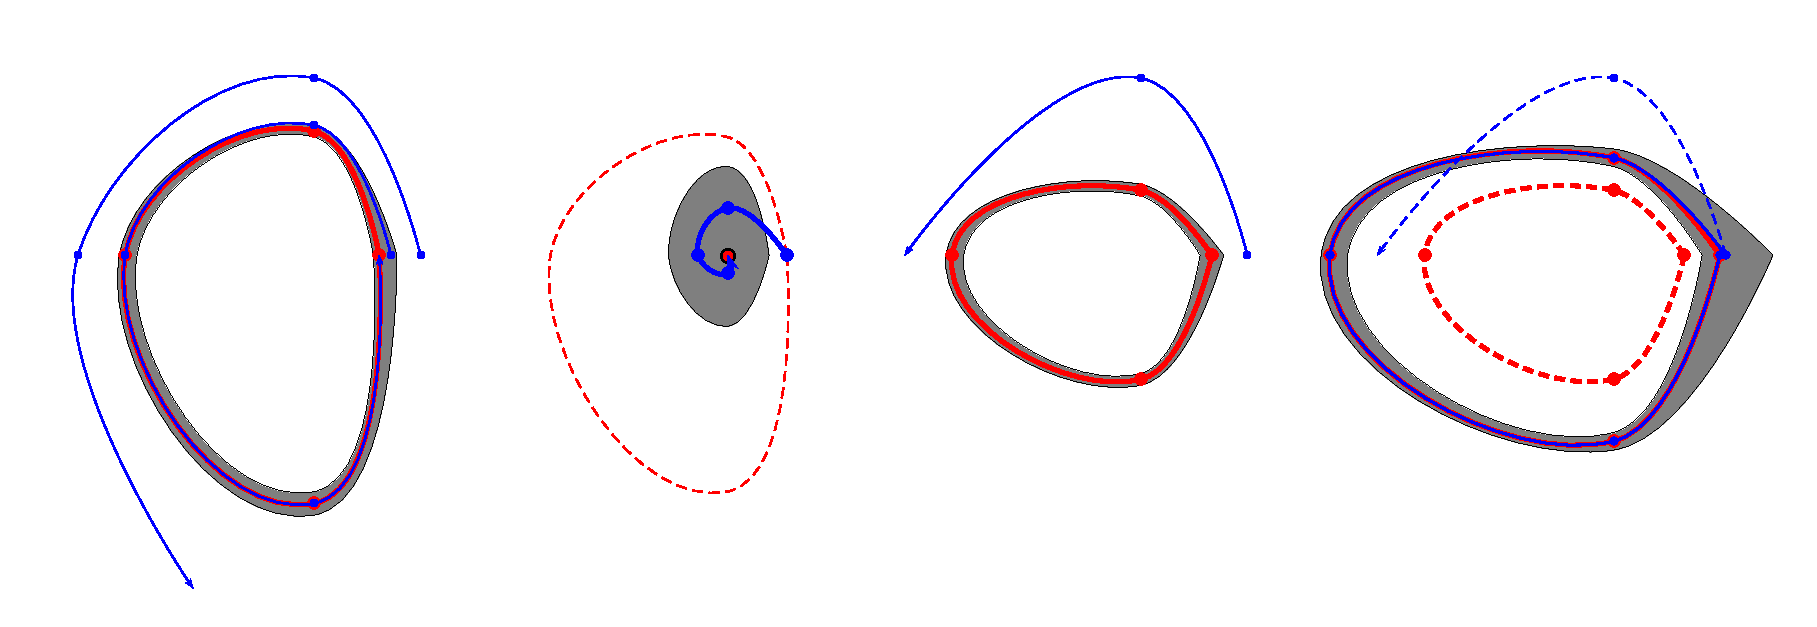
\includegraphics[width=0.7\textwidth]{LimitCircle}
    \caption{System Over View }
    \label{fig:sysoverview}
  \end{center}
\end{figure}

but when applying this method, we have condition must be met.
\begin{itemize}
\item unlike the CPG controlled example discussed in Chapter~\ref{chap:gi}.
the symmetry controlled is applied, we must prove that Symmetry Controller will not violate the topology, and symmetry control is applied to the how system rather than the original system.
We must prove that Lie Group Operator will not violate the topology

\item In chapter~\ref{chap:li} we discuss the controlled symmetry is applied to the original system, how ever, for motion synthesis, we must prove that the combined system also preserve the symmetry.
If the original system $F(x)$ have the symmetry property, we also require the neural oscillator have the same symmetry properties.
Thus we need to discuss how to transform the Neural Oscillator so the neural oscillator has the same kind of symmetry as the mechanical oscillator
\end{itemize}

the method that met the two requirements is called symmetrical entrainment control.


\subsection{Symmetrical Entrainment Control}

\begin{mythe}
Control Symmetry is Topological Conjugasim
\end{mythe}
\begin{proof}
by the definition of Lie Group

$g$ is continuous and $g^{-1}$ exist.

$g$ is isotropy.

$g$ is Topological Conjugasim

\end{proof}


We separate the discussion

after coupling with neural oscillator, the 
\[
\dot{\state}=F(\state)
\]
becomes a system 
\begin{equation}
\label{eq:gc}
\dot{\state}=F(\state)+\uout
\end{equation}
for controlled system, 
\begin{equation}
\label{eq:cc}
Tg(\dot{\state})=F(g(\state))+f_g(\uout)
\end{equation}
\begin{equation}
\label{eq:con}
\dot{state}=F(\state)+\ulocal+\uout'
\end{equation}

$f_g$ is the mapping that transform $\uout$ that make equation ~\ref{eq:gc} and ~\ref{eg:cc} satisfy the symmetry admitted by $g$
$\uout'$ is the transformed neural output,that makes the equation \ref{eq:cc} and \ref{eq:con} are equivalent.
 

as show in equation~\ref{eq:simplematsuta}.
$\uout$ is a function of $\uin$
but the system has some kinds of symmetry.
\begin{mythe}
for time scaling the input
\[
\uin(t) \mapsto \uin(\frac{t}{\alpha})
\]
if we modify the parameters $\tau_{1,2}$
\[
\tau_{1,2} \mapsto \alpha \tau_{1,2}
\]
then
\[
\uout(t) \mapsto \uout(\frac{t}{\alpha})
\]
\end{mythe}
\begin{proof}

by substitue $t'=\frac{t}{\alpha}$,$\dot{l',s'}=\alpha \dot{l,s}$,$\tau'_{1,2}=\alpha \tau_{1,2}$.


we can put the transformed parameters into equation~ \ref{eq:matsuta}, and get the same equation.

\end{proof}

based on this, we can provide an scheme to modify the parameters $\tau_{1,2}$,$\hin$,$\hout$ for maintain the symmetry of the original equation.
\begin{enumerate}
\item modify $\tau$ by the time scaling parameter $\tau \mapsto \alpha \tau$.
\item choose input variable $w$ and adjust the input efficient $\hin$ to make sure $\uin(t) \mapsto \uin(\frac{t}{\alpha})$
\item adjust the parameters of $\hout$ according to the type of driver. if $\uout$ drive the position variable $q$ then, $\hout$ should multiply by the position scale value. if $\uout$ drive the velocity,$\hout$ multiply by the speed scale parameters, if the $hout$ is force and acting on the acceleration $\ddot{q}$, then $\hout$ is multiplied by the acceleration scale value.
\end{enumerate}
Such changing parameters is call \textbf{adjoint parameter transformation} we can prove the following theorem.
\begin{mythe}
For a transformation group $G$, if modified the neural oscillator through adjoint parameters transformation, combined system will preserving permitted by symmetry $G$.
\end{mythe}
\begin{proof}
we can substitute the transformed parameters into original equation \ref{eq:cc} and find result in a equivalent equation of equation \ref{eq:gc}
\end{proof}

We can further prove that
\begin{mythe}
by apply control symmetry and adjoint parameter transformation is a topology conjugacy.
\end{mythe}
thus we maintain the structural stability of the coupled system.

Following are some examples


\subsubsection*{ Offset Symmetry.}
For offset symmetry, there is no time scaling effects.
to maintain $\uin$ and $\uout$, we require the $\uin$ and $\uout$ is a function of invariant function $I(\state)$.
For example, when walking slope changes, we choose the input of the neural oscillator to be the angle between the joints or velocity.



\subsubsection*{Time Scaling}
Neural Oscillator can change its Speed by changing $\tau \mapsto \alpha \tau $.
We prove change $ts$, we can maintain the same is maintained.
if the out is force, then it acting on the $\ddot{q}$
then $\hout \mapsto \alpha^2 \hout$

\subsubsection*{ Energy Scaling}
Energy Scaling is combined action of time scaling and pos scaling.
we can first modify the parameters $\tau$ and $\hout$ according to the speed scaling parameters.
to maintain the time scaling symmetry of $\uin$, if the input valuable is speed $\qd$, 
then $\hin \mapsto \frac{\hin}{\alpha}$ where $\alpha$ is the speed scaling value.




\subsection{Example: Height Control of Bouncing Ball}

Bouncing Ball have energy scaling symmetry, it also can also form a limit circle.
By the combined motor invariant controller, we can energy scaling the coupled system.

suppose the original system is bouncing at height of $5$
for the energy scaling, for the input to the neural oscillator is $\qd$,
then $\hin \mapsto \frac{\hin}{\alpha}$, the time scaling factor is $\alpha$, the $\tau_{1,2} \mapsto \alpha \tau_{1,2}$.
the out is the position of the pedal, so only the it need to be scale by the position scale value.for $q \mapsto \alpha^2q$,
thus $\hout \mapsto \alpha^2 \hout$.

if we set $\alpha^2=3$, then the ball will bounce at height of $15$, and it maintain its topological structure, still it is a limit cycle.
as show in figure ~\ref{fig:energy3} 


\begin{figure}[!htbp]
  \begin{center}
      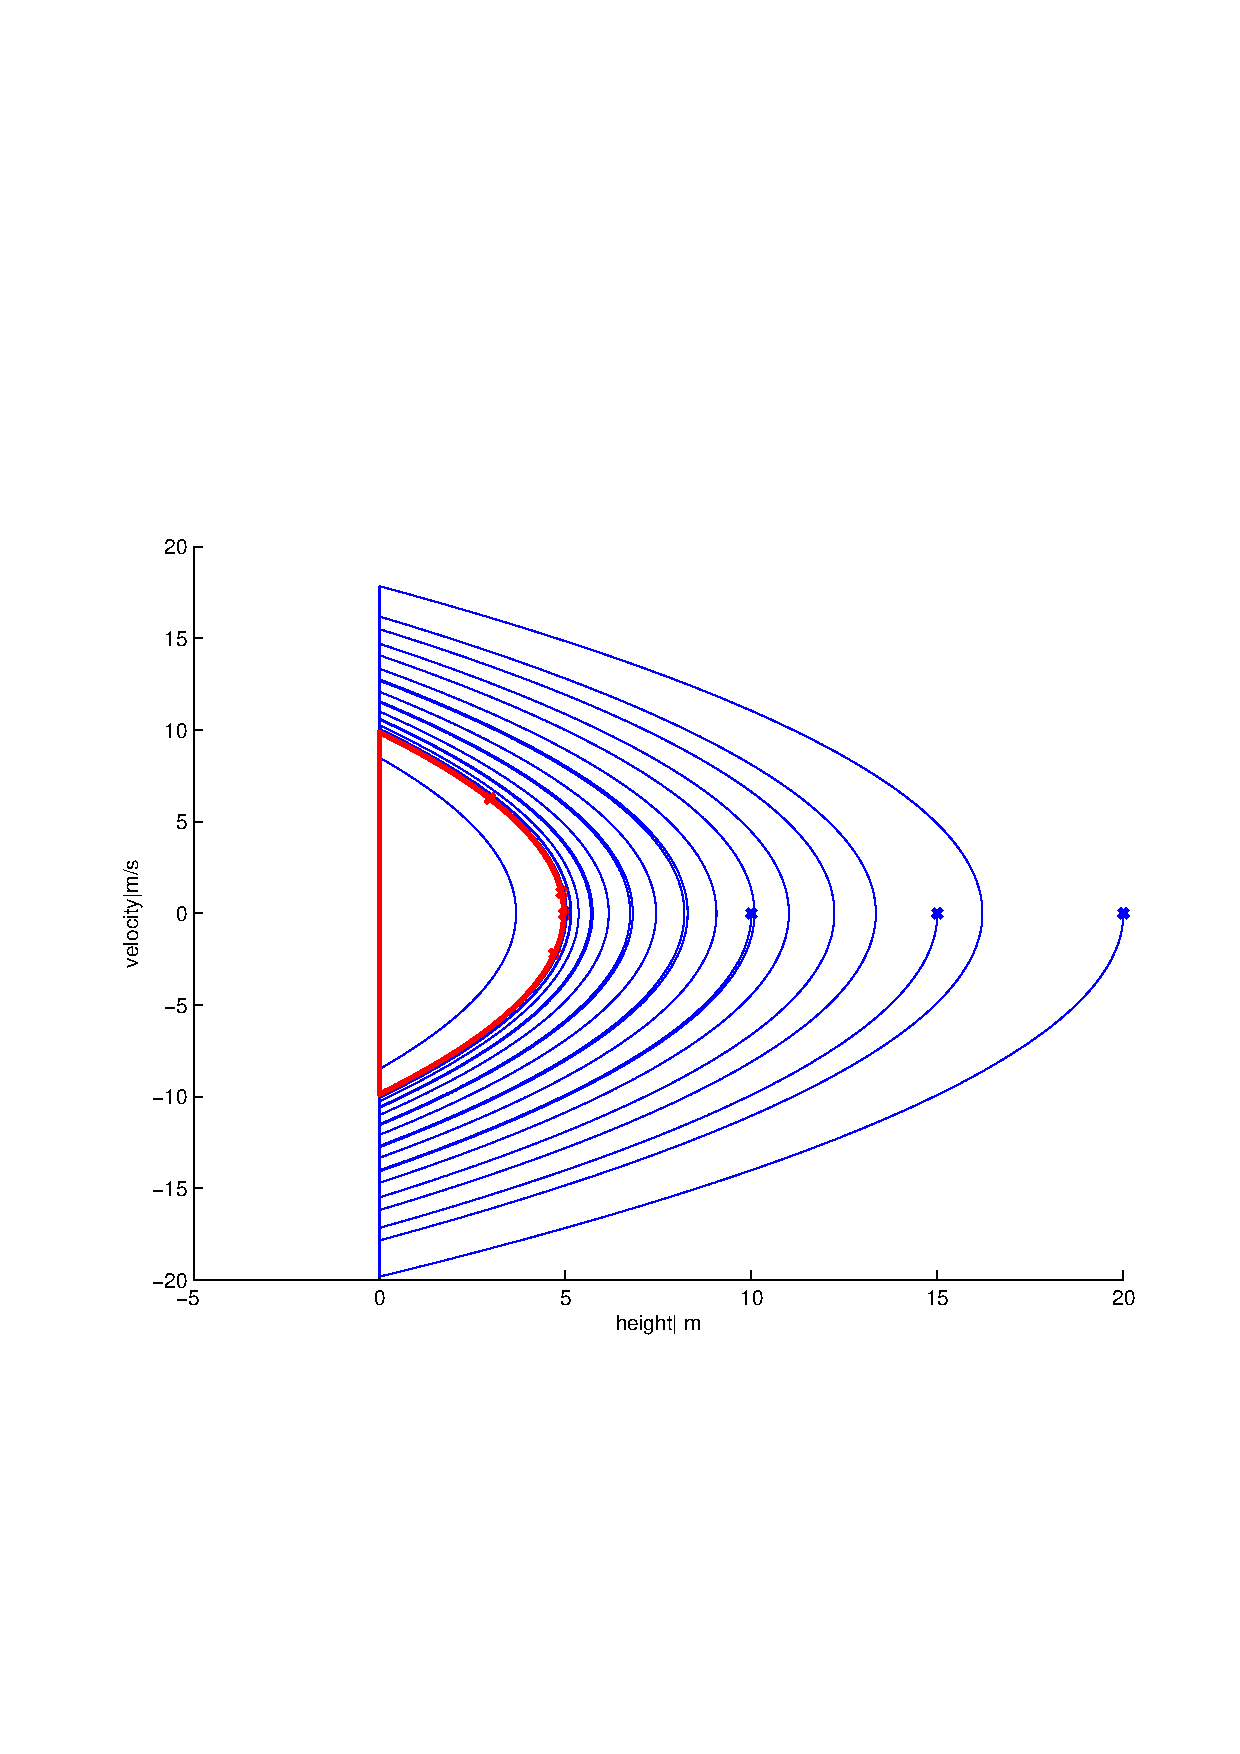
\includegraphics[width=0.7\textwidth]{BouncingBallPhasePlotAction1}
    \caption{Energy Scalling}
    \label{fig:energy1}
  \end{center}
\end{figure} 


\begin{figure}[!htbp]
  \begin{center}

      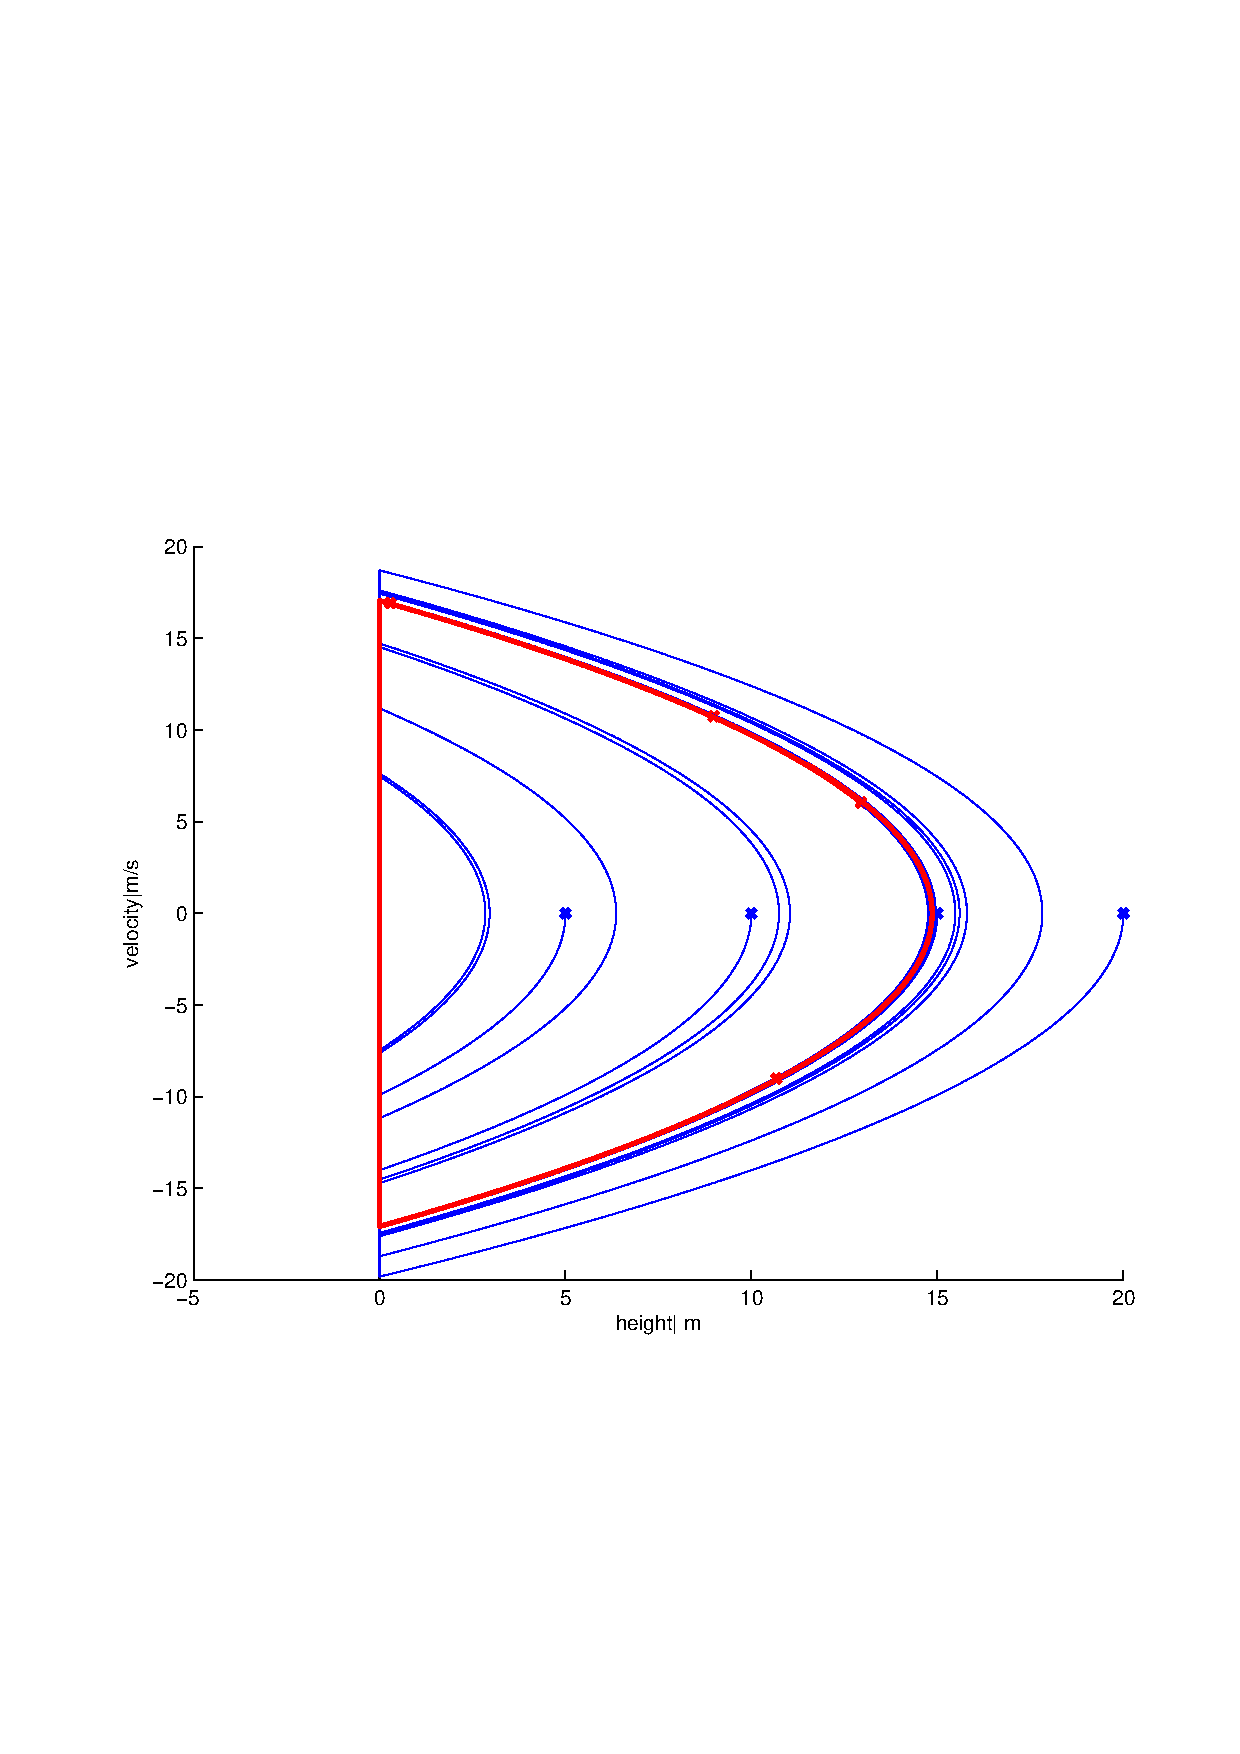
\includegraphics[width=0.7\textwidth]{BouncingBallPhasePlotAction3}
    \caption{Energy Scaling}
    \label{fig:energy3}
  \end{center}
\end{figure}

\section{Combine Motion Primitives}

\subsection{Motion Primitives Connectivity}
Motion Primitives comes from the original mechanical system, motion primitives can only transformed if they are neighbours.
Following this idea, given a dynamic system we can draw a graph of motion primitives and this is called motion primitives graph.
The idea is very similar to the motion graph, the difference here is in the original motion graph are handed crafted, 
while in our research, we propose that a motion graph of a dynamic system is fixed, at from any motion primitives, the way he can change its motion is also limited.

\begin{figure}[!htbp]
  \begin{center}
    \leavevmode
    \ifpdf
      \includegraphics[height=6in]{MotionPrimitiveGraph}
    \else
      \includegraphics[width=0.7\textwidth]{MotionPrimitiveGraph}
    \fi
    \caption{Phase Plot of Motion Primitives}
    \label{fig:manyprimitives}
  \end{center}
\end{figure}


\begin{figure}[!htbp]
  \begin{center}
    \leavevmode
    \ifpdf
      \includegraphics[height=6in]{motiongraphtopology}
    \else
      \includegraphics[width=0.7\textwidth]{motiongraphtopology}
    \fi
    \caption{Phase Plot of Motion Primitives}
    \label{fig:manyprimitives}
  \end{center}
\end{figure}


\subsection{The Motion Primitives Transition}

From dynamic point of view, changing motion primitives is put the current state into basin of attraction of another attractor.
As show in picture, for the uncontrolled system, the transition will not happen automatically, for the two basic of attraction will not overlap.

Equip with controller,
To put the state $\state$ in two different basin of attraction, we can have basically tool method.


\begin{figure}[!htbp]
  \begin{center}
    \leavevmode
    \ifpdf
      \includegraphics[height=6in]{MotionPrimitiveTransition}
    \else
      \includegraphics[width=0.7\textwidth]{MotionPrimitiveTransition}
    \fi
    \caption{Motion Primitive Transition}
    \label{fig:motion-transition}
  \end{center}
\end{figure}

\begin{itemize}
\HiItem{Overlapping Entrainment}
The first idea is use different CPG for different motion primitives. 
There is a switch mechanism of switching the CPG.
If cpg $a$ is applied to the $fx$, then the basic off attraction of $a$ is enlarged, if cpg $b$ is applied to motion primitives $b$,
the basin of attraction is also enlarged.
If a system is at a state that within the both basin of attraction, we can switch the CPG controller, we will switch the motion primitives.


\begin{figure}[!htbp]
  \begin{center}
      \includegraphics[width=0.7\textwidth]{OverLayTransition}
    \caption{Over Lay Transition}
    \label{fig:motion-transition}
  \end{center}
\end{figure}


\HiItem{Transform Method}
Controlled Symmetry can also apply for motion state transition.
For a system at $\state$, we can transform the phase portrait to make it which in the basic of attraction of $b$,
this is illustrate in figure 


\begin{figure}[!htbp]
  \begin{center}
      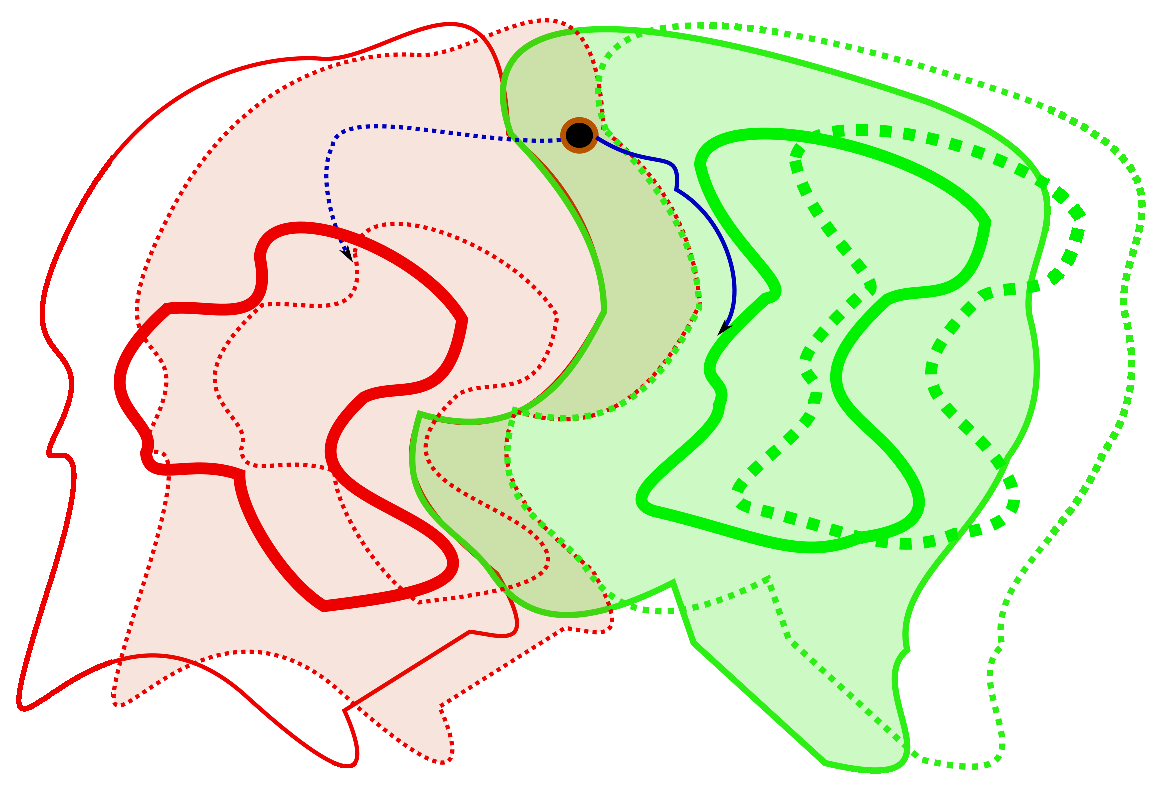
\includegraphics[width=0.7\textwidth]{OffsetTransition}
    \caption{Offset Transiton}
    \label{fig:transform-transit}
  \end{center}
\end{figure}
\end{itemize}




Both the method can result in physically realistic motion transition, when the current state $\state$ lies a special position.
The more problem happens when we don't know is where the current position x and where it is going.
Thus we combined the two methods above to achieve for a combined method,
no matter where is current point is, it is going to converge to the limit cycle, thus we ask both basic of attraction cover the limit cycle, this can be achieved via using both the CPG and Transformation.
And for this usually, both motion primitives needs to be transformed,
And the there is relationship between the two transformation; this relation ship is called transformation connection.

Figure below illustrate the idea.

\begin{figure}[!htbp]
  \begin{center}
    \leavevmode
    \ifpdf
      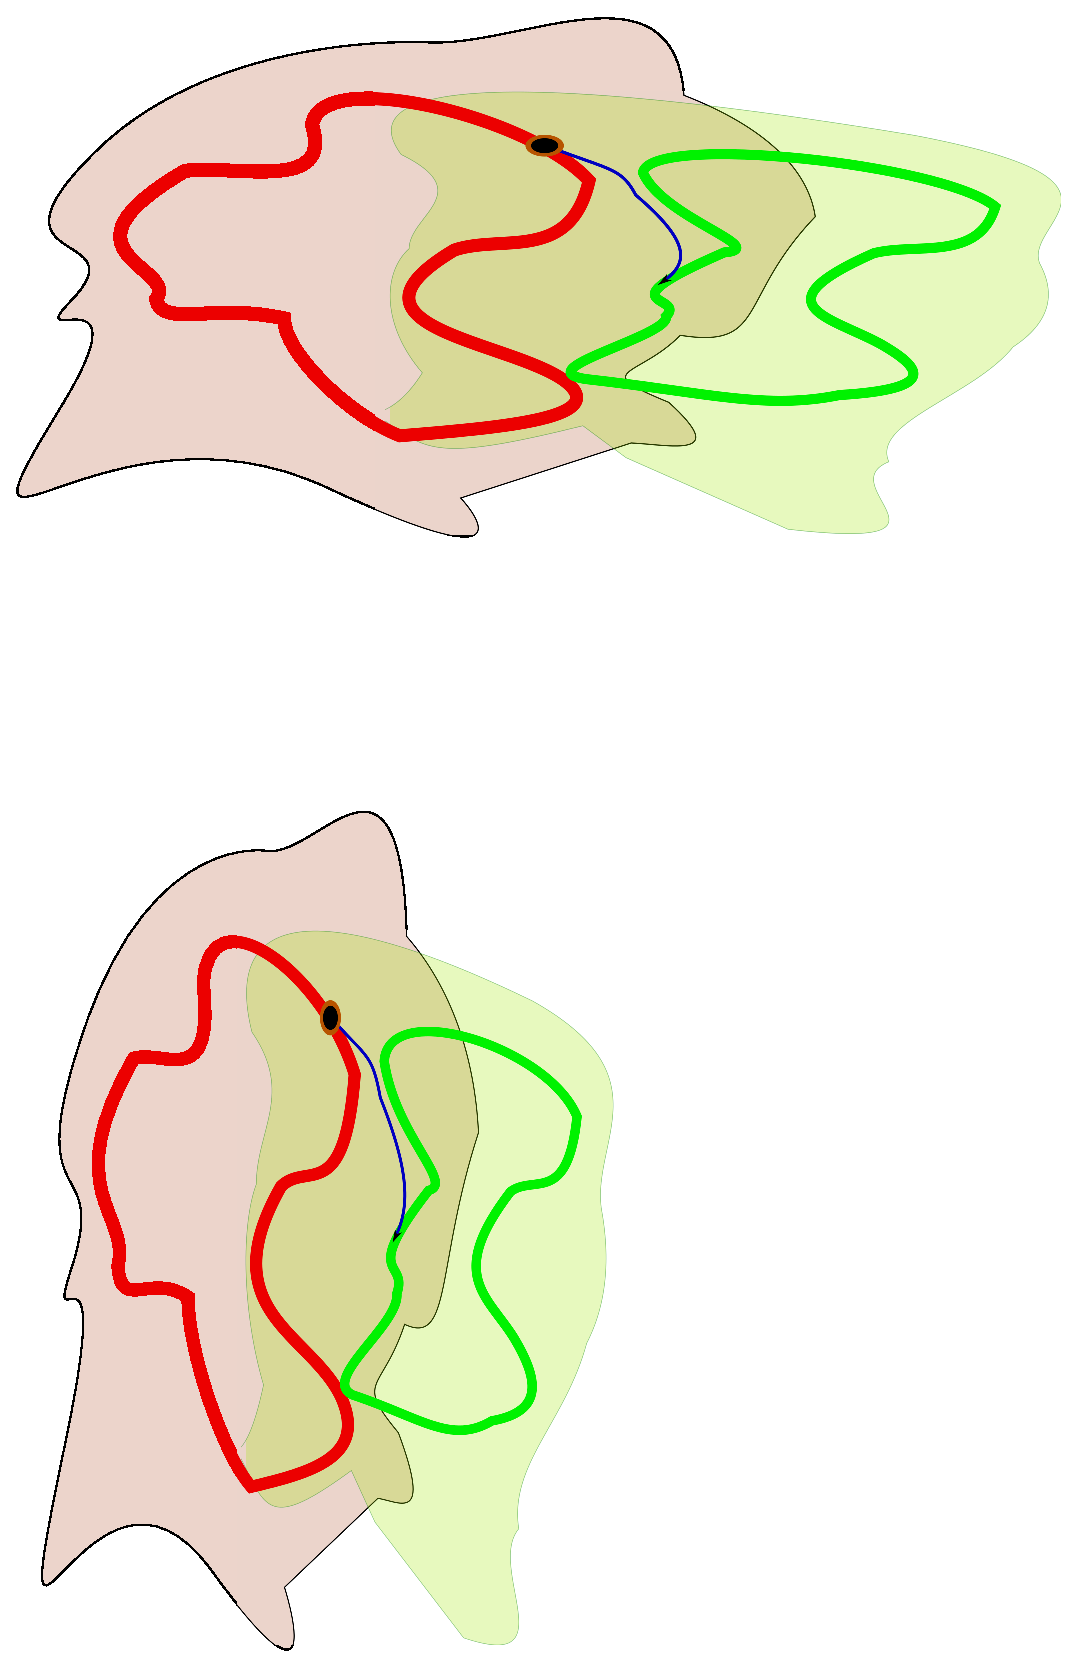
\includegraphics[height=6in]{ConbineMethod}
    \else
      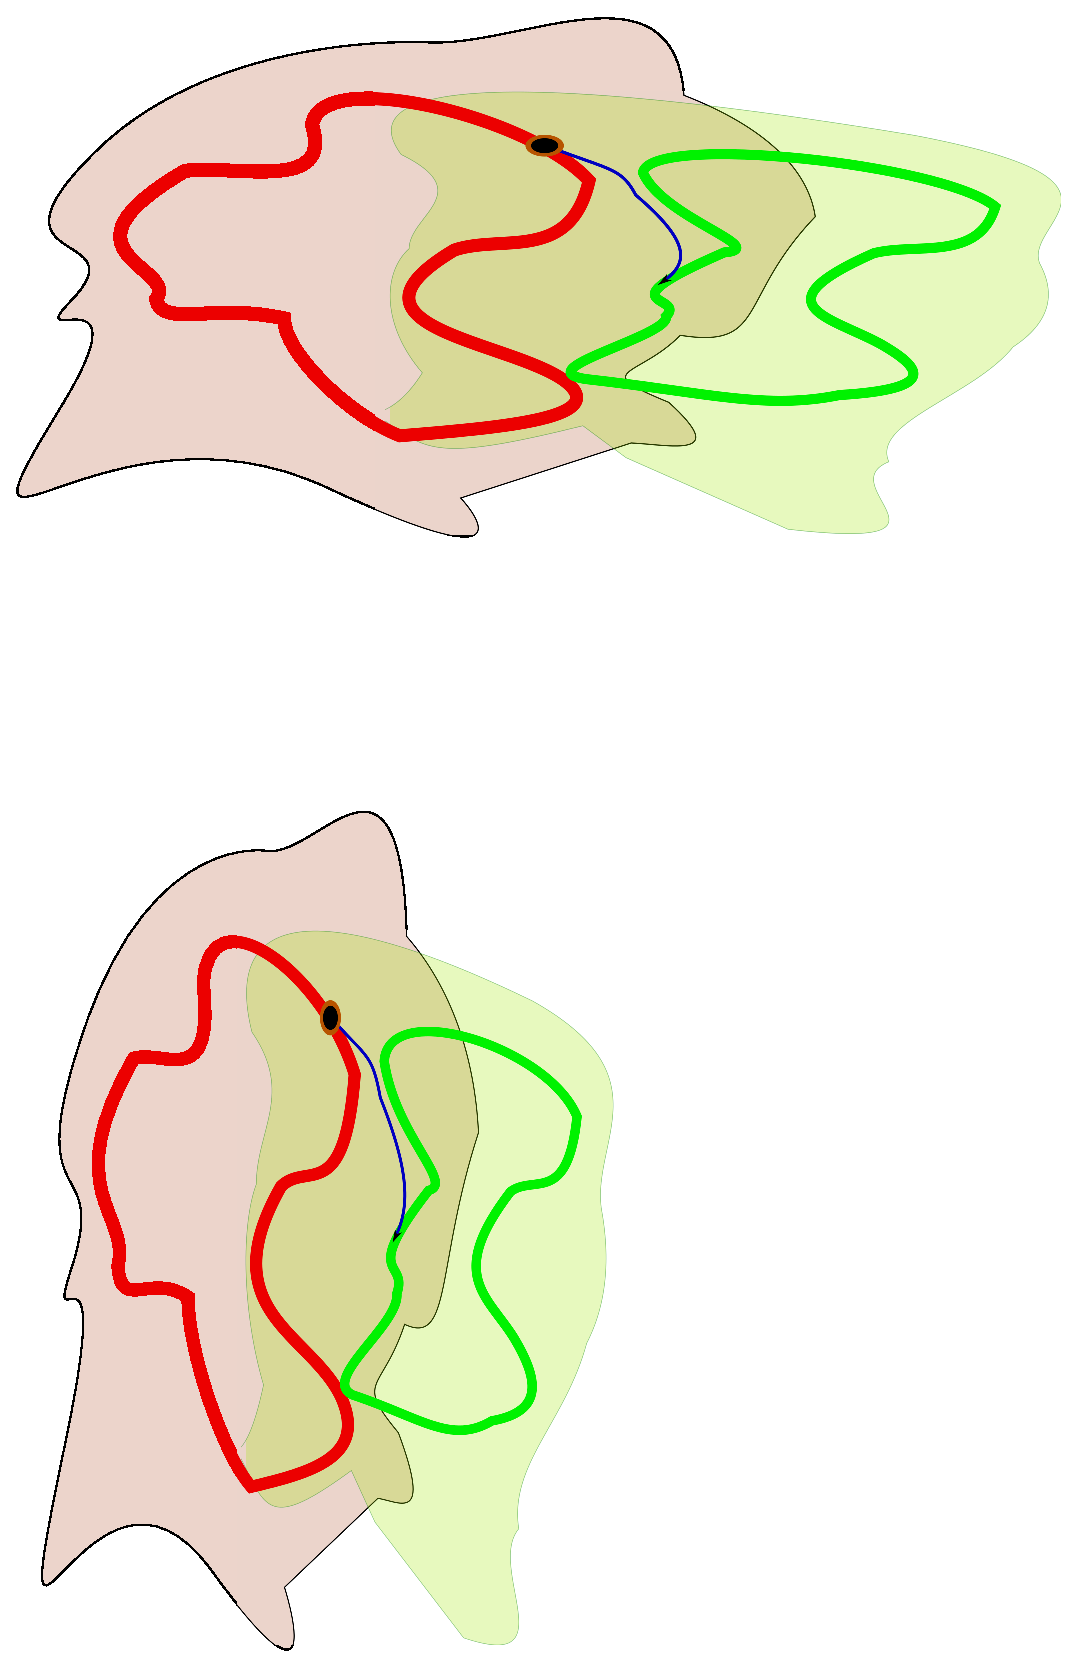
\includegraphics[width=0.7\textwidth]{ConbineMethod}
    \fi
    \caption{Comined Method}
    \label{fig:Combine}
  \end{center}
\end{figure}

\section{Motion Synthesis Framework}
While this procedure may appear mathematically complex, utilizing our approach in a motion synthesis problem is straightforward. You will need:
\begin{enumerate}
\item a mechanical oscillator $F(\x)$ which best describes the body and environment
\item a neural oscillator (for example, the Matsuoka oscillator in Equation~\ref{eq:neural_oscillator}) and associated parameters,that form a limit cycle

\item an action $g \in G$ which adapts the problem to the current environment (we present three possible operators in Section~\ref{sec:control_symmetry}). and we apply the adjoint system transformation to the neural oscillator parameters.

\item an integrator to solve the system (we use the fourth order Runge--Kutta method provided in the {MATLAB} function \emph{ode45}).
\end{enumerate}
In the following chapters ,we show how this method generates adaptive motion results.



